\documentclass[a4paper,twoside]{article}

\usepackage{epsfig}
\usepackage{subcaption}
\usepackage{calc}
\usepackage{amssymb}
\usepackage{amstext}
\usepackage{amsmath}
\usepackage{amsthm}
\usepackage{multicol}
\usepackage{pslatex}
\usepackage{apalike}
\usepackage{SCITEPRESS}     % Please add other packages that you may need BEFORE the SCITEPRESS.sty package.


\begin{document}


\title{Game to Dethrone: A Least Privilege CTF}

%%\author{\authorname{Wenjing Wu\sup{1}\orcidAuthor{0000-0000-0000-0000}, %%Second Author Name\sup{1}\orcidAuthor{0000-0000-0000-0000} and Third Author %%Name\sup{2}\orcidAuthor{0000-0000-0000-0000}}
%%\affiliation{\sup{1}Institute of Problem Solving, XYZ University, My Street, %%MyTown, MyCountry}
%%\affiliation{\sup{2}Department of Computing, Main University, MySecondTown, %%MyCountry}
%%\email{\{f\_author, s\_author\}@ips.xyz.edu, t\_author@dc.mu.edu}
%%}

\author{\authorname{Wenjing Wu, Wu-chang Feng}
\affiliation{Department of Computer Science, Portland State University}
}

\keywords{cloud security, CTF, least privilege, IAM}
\abstract
{As more businesses integrating into the cloud environment, the importance of following the principle of least privilege (PoLP) to mitigate security risks significantly increases. The fact that both identity and access management (IAM) and infrastructure itself in cloud environments are sophisticated, and the lack of CTF (Capture-the-Flag) exercises pivot around IAM best practices make the task of understanding the concepts and following PoLP onerous. This paper describes Least Privilege CTF, a series of Google Cloud based labs that can be quickly deployed at minimal cost, to assist comprehension and illustrate the process of implementing PoLP.
}

\onecolumn \maketitle \normalsize \setcounter{footnote}{0} \vfill

\section{\uppercase{Introduction}}
\label{sec:introduction}

\noindent Advantages bestowed by cloud technologies, such as efficiency, agility, scalability and cost savings, are crucial for business success in today’s market. According to the 2020 Flexera State of the Cloud Report \cite{Flexera2020}, enterprises are running 48\% of their workloads and storing 45\% of their data in public clouds and planning to increase workload and data-related cloud utilization by 9\% and 8\% respectively over the next 12 months. 

Clouds allow organizations to reduce startup costs and maintenance tasks in infrastructure (hardware and network) layers through virtualization. However, integration, both between cloud services and legacy systems and between various services from different cloud resources and platforms, is quite complex \cite{Baron2019}. 
The findings in the same Flexera report \cite{Flexera2020} indicate that 93\% of enterprises are embracing multi-cloud solutions (involving multiple public and/or private clouds), among which 87\% are taking a hybrid approach. Services from different platforms that are not always compatible with each other can pose data interoperability and ownership issues. The rapid adoption of newer technologies such as containers and serverless frameworks also contributes to cloud complexity\cite{Sharrm}. As a result, other than cloud computing itself, IAM becomes more abstruse in the cloud compared to it in legacy IT environments. The requirements to understand and configure effective access for different applications, services and platforms exacerbate the problem. 

Complicated controls and rushed technology programs, along with the shared responsibilities in cloud architecture, raise various security and privacy concerns \cite{Takabi2010}. A study \cite{Ermetic2020} commissioned by Ermetic, IDC revealed that nearly 80\% of companies experienced at least one cloud data breach during 2019 and the first half of 2020. And that the top three cloud security threats are misconfiguration of production environments (67\%), lack of visibility into access in production environments (64\%) and improper IAM and permission configurations (61\%). According to IBM's Cost of Data Breach Report 2020 \cite{IBMSecurity2020}, misconfigurations were exploited in 19\% of malicious breaches with a cost of \$4.41 million . This number is 14\% higher than the average cost of data breach.

A rash of data breaches are stemming from misconfigured or over-provisioned IAM when applying cloud services.
In the cloud breach case of Capital One during July 2019, an attacker gained identity of the EC2 instance that has privileges to access sensitive information stored in AWS S3 \cite{Parimi2019}. 
Another case was discovered from AutoClerk's unsecured Elastic search database hosted in AWS during September 2019. A surprising victim of this leak was the US government, military, and Department of Homeland Security (DHS). \cite{Fawkes2020}
In a more recent case in August 2020, Two Twitter insiders abused their excessive internal privileges to collect information of high valued users for the government of Saudi Arabia \cite{Newman2019}.

Providers and users have to carefully balance between over privilege and under privileged access \cite{Sanders2018}. Properly managing identity access and following best practices are essential of mitigating the security risk. 
In cloud computing, 

IAM ensures authentication, which validating the identity of users or systems. For example, authentication between services involves in verifying the access request to the information which served by another service \cite{AlmullaSameeraAbdulrahmanandYeun2010}.
After authentication succeeds, authorization process will determine the privileges grant to legitimate users and enforce the security policies.


The best practice regarding IAM policies is to follow the principle of least privilege(PoLP). Jerome Saltzer is accredited for the original formulation in  his paper of  Protection and the control of information sharing in multics in 1974 \cite{Saltzer1974}. The concept of PoLP is that users or processes should only have the bare minimum privileges which are indispensable to perform its intended work.

Even if PoLP is recommended by most cloud providers for security reason, many companies find it difficult to prioritize or practice in development. 
As mentioned earlier, cloud systems are now so complex that developers are reluctant to modify the settings once "it works". As a consequence, the security gaps created by layers or new technologies will rarely or never be patched. A report on DevOps security has found that only 4\% of issues found in production are dealt with after development \cite{Foremski}. 
An interesting case study is that cloud service provider sometimes suggests using Owner role that granted with maximum permission in their documentation (Quickstart: Setup the Vision API) \cite{GoogleVis}. Based on the developer behavior we know, this could generate a potential attacking surface in the future.
Developers need guidance or training for secure coding, however, nearly 70\% of developers expressed that they get little help in GitLab's 2019 Global Developer Report  \cite{Gitlab2019}.

The principle of least privilege is essential to cloud security. There are many cloud CTF exercises available online covering a wide variety of vulnerabilities. Most of them are AWS (Amazon Web Services) based \cite{flaws} \cite{flaws2} \cite{cloudgoat} \cite{serverlessgoat}, only two of them contain  GCP (Google Cloud Platform) based exercises \cite{thunder-ctf} \cite{QWIKLABS}.  However, none of them is destined for the purpose of training developers on how to implement PoLP in cloud environment. To address this, we create Least Privilege CTF, a set of CTF exercises for helping practice and implement PoLP on Google Cloud Platform.

Section 2 furnishes the definition of identity and access control in Google Cloud. Section 3 describes the comprehensive design of Least Privilege CTF and its levels. Section 4 exhibits the results of an initial deployment in an advanced elective course in our program. Lastly, Section 5 presents related work and section 6 concludes.


\section{\uppercase{Google Cloud IAM}}
\label{sec:gcpiam}

\noindent Identity and Access Management provides protection for resources and data through rules and policies which are enforced on users via various techniques. Common ones are enforcing login passwords, assigning privileges to the users and provisioning user accounts \cite{AlmullaSameeraAbdulrahmanandYeun2010}.
Similarly, in Google Cloud, IAM grants granular access to specific resources and helps prevent access to other resources \cite{Googlecloudiam}.

Identities are essentially authenticated members. A member (Figure~\ref{fig:mem}) can be a Google Account for end users (userid@gmail.com), a service account for apps and virtual machines (12345678@cloudservices.gserviceaccount.com), a Google group (groupname@googlegroups.com), or a G Suite or cloud identity domain that can access a resource (alias@example.com). The identities of the first three member types are email addresses. The identity associated with G Suite or cloud identity domain is usually a domain name.
\begin{figure}[h]
  \centering
  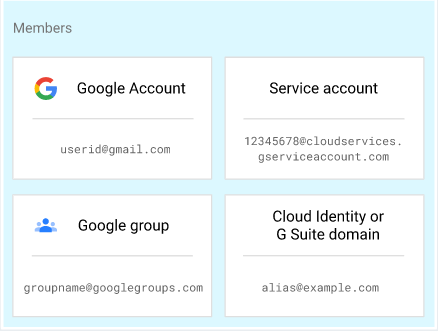
\includegraphics[width=\linewidth]{pic/mem}
  \caption {Types of Members in GCP}
  \label{fig:mem}
\end{figure}

An authorization process that grants access of resources to members can be achieved through role and policy. A role is a collection of permissions determining what operations are allowed on a resource (Figure~\ref{fig:role}). Instead of assigning permissions directly to end users, in Google Cloud, permissions are grouped into roles and then granted to authenticated members to access resources. Granting a role to a member actually grants all the permissions of that role.
\begin{figure}[!h]
  \centering
  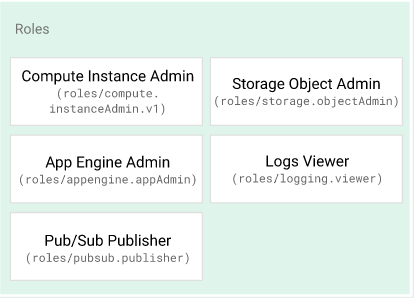
\includegraphics[width=\linewidth]{pic/role}
  \caption {GCP Predefined Role}
  \label{fig:role}
\end{figure}
A policy binds who (member) has what access (role) for which resource \cite{Googlecloudiam}. Some examples of resources are organizations, folders, projects, Compute Engine instances, and Cloud Storage buckets. The binding between members and roles is a many-to-many relationship.
Primitive, predefined, and custom roles are three types of roles supported in Google Cloud IAM \cite{googlecloudrole}. Primitive roles (renamed as Basic roles later) comprises Owner, Editor and Viewer roles, which exist prior to the introduction of IAM in GCP. For example, the account one uses to create a project will be automatically attach with Owner role. Predefined roles are finer-grained roles for a particular service or resource. Privileges can also be limited further by creating a custom role and attach permissions across services based on user selection. Unfortunately, not all permissions can be linked to Custom roles such as Datastore related permissions. 

The role based model of cloud IAM simplifies the implementation of PoLP. To illustrate this, we can take the access control of Cloud Storage as an example. In Cloud Storage, everything that must be contained in a bucket. Buckets are the basic containers that hold objects such as files, images, etc. Suppose in a project, a set of users need access to view files and file content in a public bucket. For beginners, an easy solution is to create a Google group for the users and grant Storage Admin role (roles/storage.admin) to it. However, looking through Table~\ref{table:sto-role}, which demonstrates all predefined Cloud Storage roles and corresponding permissions, it is obvious that Storage Object Viewer role would be sufficient for users to perform the same task. 
\begin{table}[t]
    \caption{IAM roles for Cloud Storage} \centering
    \begin{tabular}{|p{4.2cm}|p{4cm}|}
    \hline
    Role & Permissions\\
    \hline
    \hline
    Storage Object Creator\par(roles/storage.objectCreator) &  resourcemanager.projects.get \par resourcemanager.projects.list \par storage.objects.create \\ %% $\pm$ \\
    \hline
    Storage Object Viewer\par(roles/storage.objectViewer) & resourcemanager.projects.get\par resourcemanager.projects.list\par storage.objects.get\par storage.objects.list \\ %% $\pm$ \\
    \hline
    Storage Object Admin\par(roles/storage.objectAdmin) & resourcemanager.projects.get \par resourcemanager.projects.list\par storage.objects.*\\ %% $\pm$ \\
    \hline
    Storage HMAC Key Admin\par(roles/storage.hmacKeyAdmin) &storage.hmacKeys.*\\
    \hline
     Storage Admin\par(roles/storage.admin) &firebase.projects.get\par resourcemanager.projects.get\par resourcemanager.projects.list\par storage.buckets.*\par storage.objects.*\\
    \hline
    \end{tabular}
    \label{table:sto-role}
\end{table}
Therefore, Storage Object Viewer role is a better option (Figure~\ref{fig:sto-pre}), but still it is over-privileged. 
\begin{figure}[!h]
  \centering
  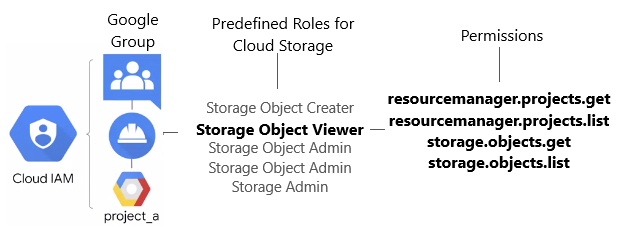
\includegraphics[width=\linewidth]{pic/sto-pre}
  \caption {Policy - Predefined Role}
   \label{fig:sto-pre}
\end{figure}
Google documentation explains that storage.objects.list and storage.objects.get are actual permissions that allow a member to list files and view file content. To follow PoLP and optimize the solution, we can create a custom role with the two least privileges attached and bind the custom role to the Google group(Figure~\ref{fig:sto-cus}).
\begin{figure}[!h]
  \centering
  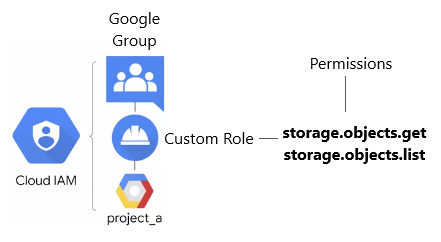
\includegraphics[width=\linewidth]{pic/sto-cus}
  \caption {Policy - Custom Role}
   \label{fig:sto-cus}
\end{figure}


\section{Least Privilege CTF}
\subsection{Design Goal}
The purpose of building Least Privilege CTF is to effectively teach developers about how IAM works and how to adopt PoLP in GCP. Meanwhile, the CTFs should be able to run at minimum cost and fast, deliver instant feedback, extensible, friendly to beginners and scaffolding.
\begin{enumerate}
\item Minimum cost: Anyone can apply for 300 credits(dollars) for free with a Google account and credit card. If levels are deleted upon completion, monthly cost would be less than a dollar (Figure~\ref{fig:cost}). 
\begin{figure}[!h]
  \centering
  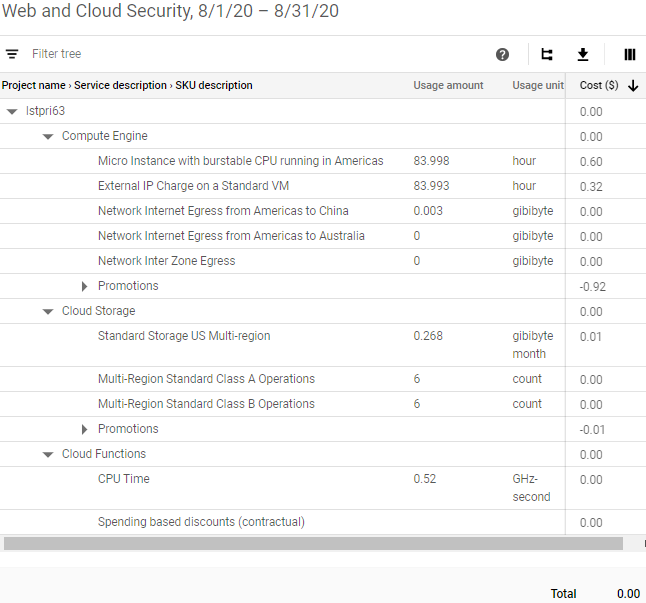
\includegraphics[width=\linewidth]{pic/cost}
  \caption {Billing - Monthly Cost}
  \label{fig:cost}
\end{figure}
\item Fast Deployment:  Deploy initial 11 levels in 4.5 minutes.
\item Extensible: Easy to add new level with simple modification. 
\item Beginners friendly: Explicit and detailed instructions are available in the UI for every level. Prior Google Cloud knowledge is optional.
\item Instant feedback: Results will show up immediately along with failing reason for each attempt.
\item Scaffolding: Differentiated and incremented level difficulties for the benefit of both novices and experienced practitioners.

\end{enumerate}

\subsection{Implementation}

\subsubsection{Thunder CTF and Modular}
Least privilege CTF is developed based on Thunder CTF, a scaffolded, scenario-based CTF that helps students learn about and practice cloud security skills on GCP. Each Thunder CTF level includes a yaml development configuration, a python deployment script and an HTML content for hints \cite{Springer}. The modular design and specific structure reduces the process of adding new levels to simply filling in a template. Least privilege CTF inherits the modular structure from Thunder CTF with modification. Rather than deploy each level individually, Least Privileges CTF deploys all required resources specified in the yaml file at one time in parallel with Google Cloud Deployment Manager, which takes about 4.5 mins for 11 levels.

\subsubsection{UI and Cloud Functions}
Despite a page \cite{lst-ctf} hosted under main Thunder CTF website for steps of environment set-up and initial deployment, Least Privilege CTF does not generate level hints with HTML contents or render scripts in a similar way as in Thunder CTF. Instead, the hints system is replaced by Cloud Function \cite{cloudfunc}, a pay-as-you-go service that automatically scales based on loads. There are several advantages comes from Cloud Function. First, services only get billed for execution time. Second, Cloud Functions demand no server management which speeds up the development as we do not have to deal with the operational infrastructure in Google Cloud. Third, Cloud Function integrates with logging and debugging capabilities, making the coding experience intuitive. Last, the service has built-in security based on PoLP at role per function. 

The type of function to create level instructions and hints in Least Privilege CTF is HTTP function. HTTP functions are invoked by standard HTTP requests and supports common methods like GET, PUT, POST, DELETE and OPTIONS \cite{httpfunc}. A typical procedure in our design framework is that when a function is triggered by events, it waits for responses either returned from a Cloud service or submitted in front-end using POST or GET method. Thanks to the TLS certificates that automatically provisioned in Cloud Functions service, all HTTP functions can be invoked with a secure connection. 

In order to call a function and pass parameters, an URL known as HTTP-Triggered-Endpoint is obtained after each function deployment. Figure~\ref{fig:endpoints} shows the function endpoints printed in Cloud Console shell when deployment manager completes the operation and creates initial levels. In Least Privilege CTF, functions are written in python and interact with other cloud services through APIs. The returned results of a function will be rendered into HTML through Jinja and appear in the form of a web page. Players can access the page in web browser via related function endpoint.

Each level contains two functions, an access function (Figure~\ref{fig:access}) and a check function (Figure~\ref{fig:check}). In the UI created with access function, players can find level resources, step by step instructions towards completion and a code snippet that helps figure out what the function does. The check function lists current roles and permissions that a player choose as the answer and displays the validation result. In addition,  a Scoreboard Function is implemented to keep track of the overall accomplishment of all levels (Figure~\ref{fig:score}).  
\begin{figure}[!h]
  \centering
  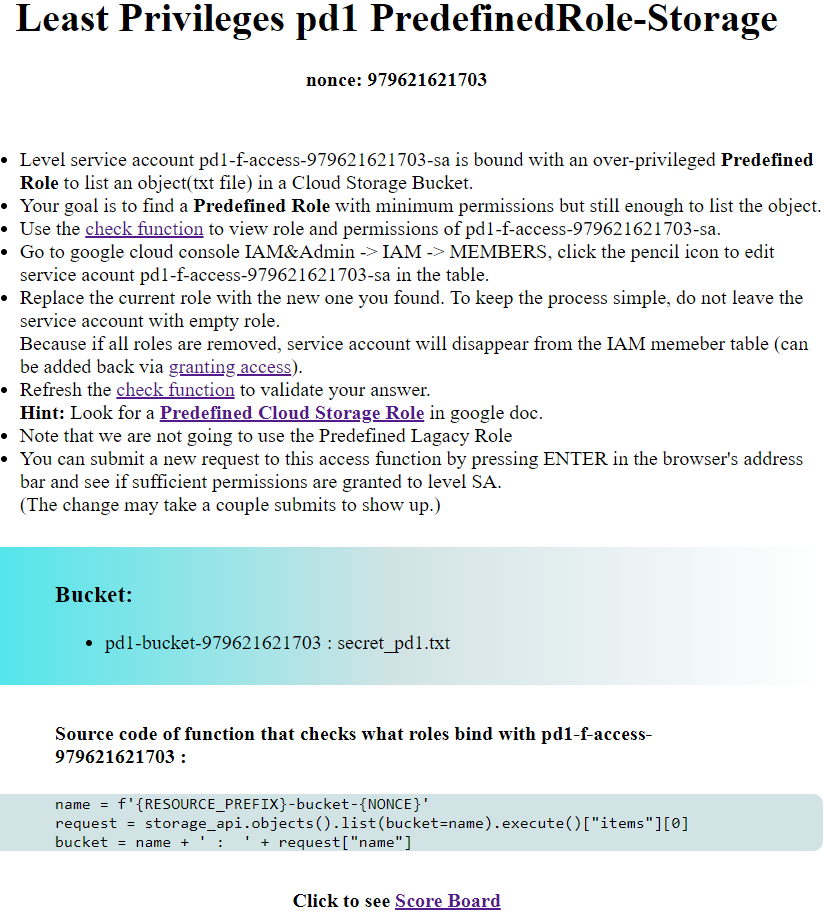
\includegraphics[width=0.5\textwidth]{pic/access}
  \caption {Access Function}
  \label{fig:access}
\end{figure}
\begin{figure}[!h]
  \centering
  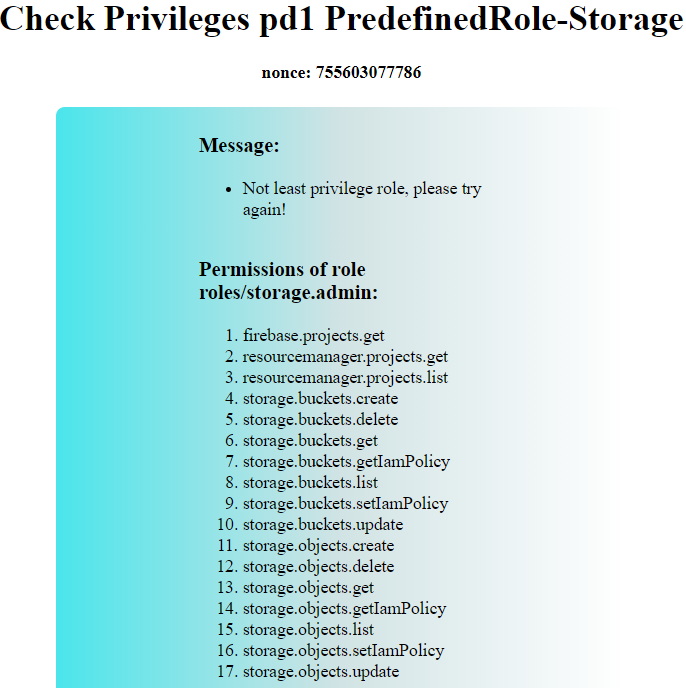
\includegraphics[width=0.5\textwidth]{pic/check}
  \caption {Check Function}
  \label{fig:check}
\end{figure}

\begin{figure}[!h]
  \centering
  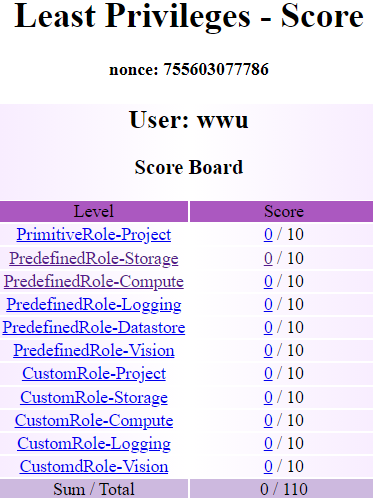
\includegraphics[width=0.4\textwidth]{pic/score}
  \caption {Scoreboard Function}
  \label{fig:score}
\end{figure}

\begin{figure*}[h]
  \centering
  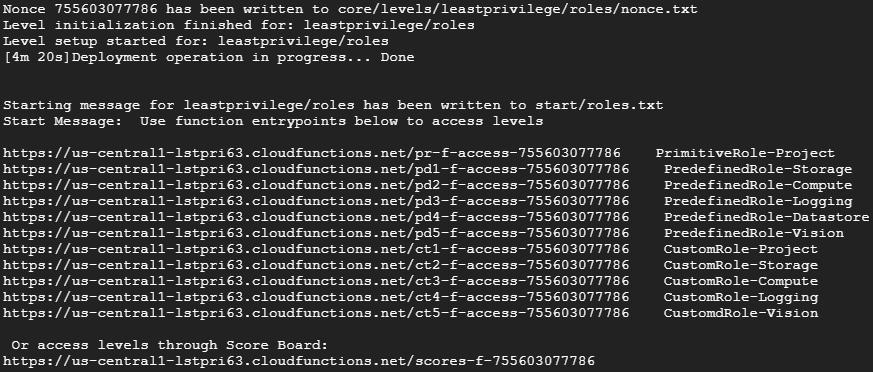
\includegraphics[width=0.7\textwidth]{pic/endpoints}
  \caption {Endpoints}
   \label{fig:endpoints}
\end{figure*}
%%\begin{figure*}[t]
%%  \centering
 %% \begin{tabular}{c}
 %% 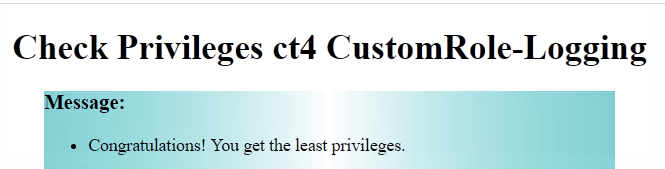
\includegraphics[width=0.60\textwidth]{success}
%%  \end{tabular}
%%\caption{Figure 1: function-validate answer and provide hints}
%%\label{fig:hints}
%%\end{figure*}
\subsubsection{Levels}
There are eleven levels implemented in Least Privilege CTF so far, and they are designed in a scaffolded style with incrementally increasing difficulties. The type of role and service that each level targets on are implied in level name and joined by a dash (first column of Figure~\ref{fig:score}). 

In the design of Least Privilege CTF, all functions are expected to access level resources only with their default identities, the service accounts created and attached during deployment. The roles bind with these service accounts can be updated after deployment in Google Cloud Console. 
A check function validates whether the binding role(s) in access function matche(s) the correct answer, so a role with permissions to list and get roles or IAM policy is always required. The score board function is using similar technique to validate answers and calculate scores, and repeat this for all levels. The roles bind with access functions are more complicated and vary based on specific levels. In general, access functions begin with a role of excessive permissions to perform certain actions described in level instruction. The winning condition is to apply PoLP and grant minimum privileges that are just enough to perform the same action. The process of picking and specifying more restrictive roles has been exemplified in Section~\ref{sec:gcpiam}.

Players may spend a little bit more time on the levels regarding Cloud Vision service - a service that does not have a set of predefined roles or permissions associated in GCP, indicating that the authenticated service accounts will have default access to Cloud Vision API. In order to analyse images with Cloud Vision service, the players are required to upload images into a Bucket through the form in front-end page (access function). The analysed results will be inserted into Cloud Datastore and listed in the same page.  The roles or permissions to complete such tasks are actually in Cloud Storage and Datastore category. The correct answer of level CustomRole-Vision is a combination of predefined role and custom role. As mentioned in Section~\ref{sec:gcpiam}, GCP does not support Datastore permissions in Custom Role yet.
 

\section{Evaluation}
 \noindent The first use of Least Privilege CTF occurred in our Fall 2020 offering of Portland State University's CS 430/530 Internet, Web, and Cloud Systems course with 60 students.  The first half of the 10-week course covers key concepts in networking, operating systems, web development, and databases before transitioning to their use in cloud computing environments. At the beginning of the 5th week, a lecture on Google Cloud Identity and Access Management is given to students and the Least Privilege CTF levels were assigned. Students were given a due date for the exercises at the end of the 5th week, allowing them about a week to finish the levels.

To assess the effectiveness of the CTF, we surveyed students at the beginning of the 10th week. Below we list the questions that were asked in the survey in bullet points.  Our goal was to measure how well the CTF helped students learn about cloud security issues related to IAM and understand best practice.  

Questions included in the survey:
\begin{itemize}
\item Q1: Rate the exercise for helping to understand least-privilege access control issues in the cloud.
\item Q2: Rate the exercise for helping to develop skills for applying the principle of least-privilege access control in the cloud.
\item Q3: Rate the scaffolding of levels in the exercise for helping to quickly learn about least-privilege access control in the cloud.
\end{itemize}

Of the 60 students in the class, 36 responded to the survey.  Table~\ref{table:data} shows the results. As the table shows, students felt that the lecture material and CTF exercises were both helpful for learning Cloud IAM and the principle of least privilege, while students found the scaffolded levels and instructions very helpful as a learning aid, validating our design.

\begin{table}[h]
 \vspace{-0.20cm}
 \caption{Helpfulness ratings of Least Privilege CTF (1=Very Unhelpful, 2=Somewhat Unhelpful, 3=Neither Helpful nor Unhelpful, 4=Somewhat Helpful, 5=Very Helpful)}
    \label{table:data} \centering
    \begin{tabular}{|c|c|c|c|c|c|c|}
    \hline
    Question & 1 & 2 & 3 & 4 & 5 &Mean rating\\
    \hline
    \hline
    Q1 & 1 & 3 & 3 & 19 & 10 & 3.94\\ %% $\pm$ \\
    \hline
    Q2 & 1 & 2 & 4 & 20 & 9 & 3.94\\ %% $\pm$ \\
    \hline
    Q3 & 1 & 0 & 1 & 10 & 24 & 4.56\\ %% $\pm$ \\
    \hline
    \end{tabular}
\end{table}



\section{Related Work}

\noindent Developers and researchers have actively worked on building cloud security CTF exercises or labs. Existing AWS CTF platforms are consist of  Flaws \cite{flaws}, Flaws2 \cite{flaws2}, CloudGoat \cite{cloudgoat} and OWASP ServerlessGoat \cite{serverlessgoat}. These platforms demonstrate common security issues caused by various reasons throughout development, including authentication bypass and over-privileged access(misconfigured IAM). Most CTF exercises are offensive style, meaning the player will act as an attacker. It is the players’ mission to identify vulnerabilities, and exploit the way to the ‘secret’. Flaws2 contains both offensive and defensive style of CTF. Thunder CTF \cite{thunder-ctf} covers an extensive range of GCP based labs, however best practice is not designed in any level. QWIKLABS \cite{QWIKLABS} seems to be the only platform that builds security labs regarding both AWS and GCP. Their courses and labs aim to help users gain cloud knowledge, practice building projects and get familiar with cloud services as quickly as possible. Although some QWIKLABS projects do require creating service account, attaching roles and granting permissions, they issue temporary cloud credentials for players, so security has never been their main concern.

Existing services are available to help achieve PoLP with less effort by monitoring logs and configuration. For example, Google IAM Recommender \cite{GoogleLstRec} provides safe, in-context, and actionable changes to IAM policies that move a project towards PoLP and don’t require lots of manual effort. However, it will have to gather enough data to be able to make suggestions. This limitation makes Google IAM Recommender as well as a lot of other third party tools impractical for education purposes.

\section{\uppercase{Conclusions}}
\label{sec:conclusion}

\noindent Identity and access management and following best practice are imperative in cloud security, however the concept of IAM and PoLP is difficult to understand. In this paper, we designed and implemented CTF exercises focused on enforcing the principle of least privilege in Google Cloud IAM. The evaluation showed that results from an initial offering are promising and the design goals are achieved. 

\section*{\uppercase{Acknowledgments}}
\noindent This material is supported by the National Science Foundation under Grant No. 1821841. Any
opinions, findings, and conclusions or recommendations expressed in this material are those of the author and do not necessarily reflect the views of the National Science Foundation.


\bibliographystyle{apalike}
{\small
\bibliography{ref-base}}




\end{document}

